\documentclass[11pt,a4paper]{article}
\usepackage[margin=2.2cm]{geometry}
\usepackage{amsmath}
\emergencystretch=5em
\usepackage{microtype}
\usepackage{graphicx,listings,xcolor,booktabs,longtable,array,hyperref,enumitem}
\usepackage{tikz}\usetikzlibrary{shapes.geometric,arrows.meta,positioning}
\hypersetup{colorlinks=true,linkcolor=blue!50!black,urlcolor=blue!50!black}
\lstset{basicstyle=\ttfamily\footnotesize,breaklines=true,frame=single,
  keywordstyle=\color{blue!60!black},commentstyle=\color{green!40!black},
  language=C++,numbers=left,numberstyle=\tiny,columns=fullflexible}
\newcommand{\todo}[1]{\textcolor{red}{\textbf{[FILL IN: #1]}}}
\title{\textbf{Skill Issue -- A Peer-to-Peer Skill Exchange Platform}\\[2pt]
\large CSLR31 Data Structures Laboratory -- Project Report}
\author{\textbf{Team: All H's}\\[4pt] 106125037 -- Harini\\ 106125039 -- Harsh\\ 106125041 -- Himani}
\date{\today}
\begin{document}
\maketitle
\tableofcontents
\newpage

%=====================================================================
\section{Step 1 -- Problem Identification (Abstract)}
\textbf{Title:} Skill Issue -- A Peer-to-Peer Skill Exchange Platform.

\noindent\textbf{Problem and motivation.} Students on a campus hold very different skills (programming, music, dance, languages), yet there is no simple way to find a peer who can teach a skill, agree on a time, and be recognised for teaching. Paid courses are expensive and generic, so many students stay stuck on a skill they could learn from a classmate. This supports UNESCO/UN \textbf{SDG~4 (Quality Education)} by making peer learning accessible and free.
\textbf{Existing products} such as Coursera, Udemy and Superprof are paid or one-directional marketplaces; campus WhatsApp groups are unstructured and keep no record of sessions or reputation.
\textbf{Objectives:} let users register their teachable skills, find mentors for a skill, request and schedule sessions, track attendance, and reward good teaching.
\textbf{Salient features:} (i) skill-based mentor matching ranked with a hand-written stable merge sort; (ii) a booking life-cycle (PENDING $\rightarrow$ OFFERED $\rightarrow$ CONFIRMED $\rightarrow$ session) with mentor time offers; (iii) attendance reporting with no-show disputes resolved by an admin; (iv) points system (learner ratings and quiz scores) feeding a teaching leaderboard; (v) self-written hash map for $O(1)$ look-ups and a self-written heap for top-$k$ mentors; (vi) CSV persistence, a console interface and a REST API consumed by a React web front end.
\textbf{Future scope:} a skill graph with trie-based skill search, interval-based time-slot conflict detection with a request queue, password hashing, notifications, a database back end and mobile support.

%=====================================================================
\section{Step 2 -- Design of the Product}
Figure~\ref{fig:flow} shows the flow chart of the main workflow. Grey boxes mark the steps where a data structure or algorithm does the real work. (If \texttt{figures/flowchart.pdf}, exported from \texttt{flowchart.dot}/\texttt{.fig}, is present it is used; otherwise the built-in diagram below is drawn, so the report always compiles.)
\begin{figure}[p]\centering
\IfFileExists{figures/flowchart.pdf}{%
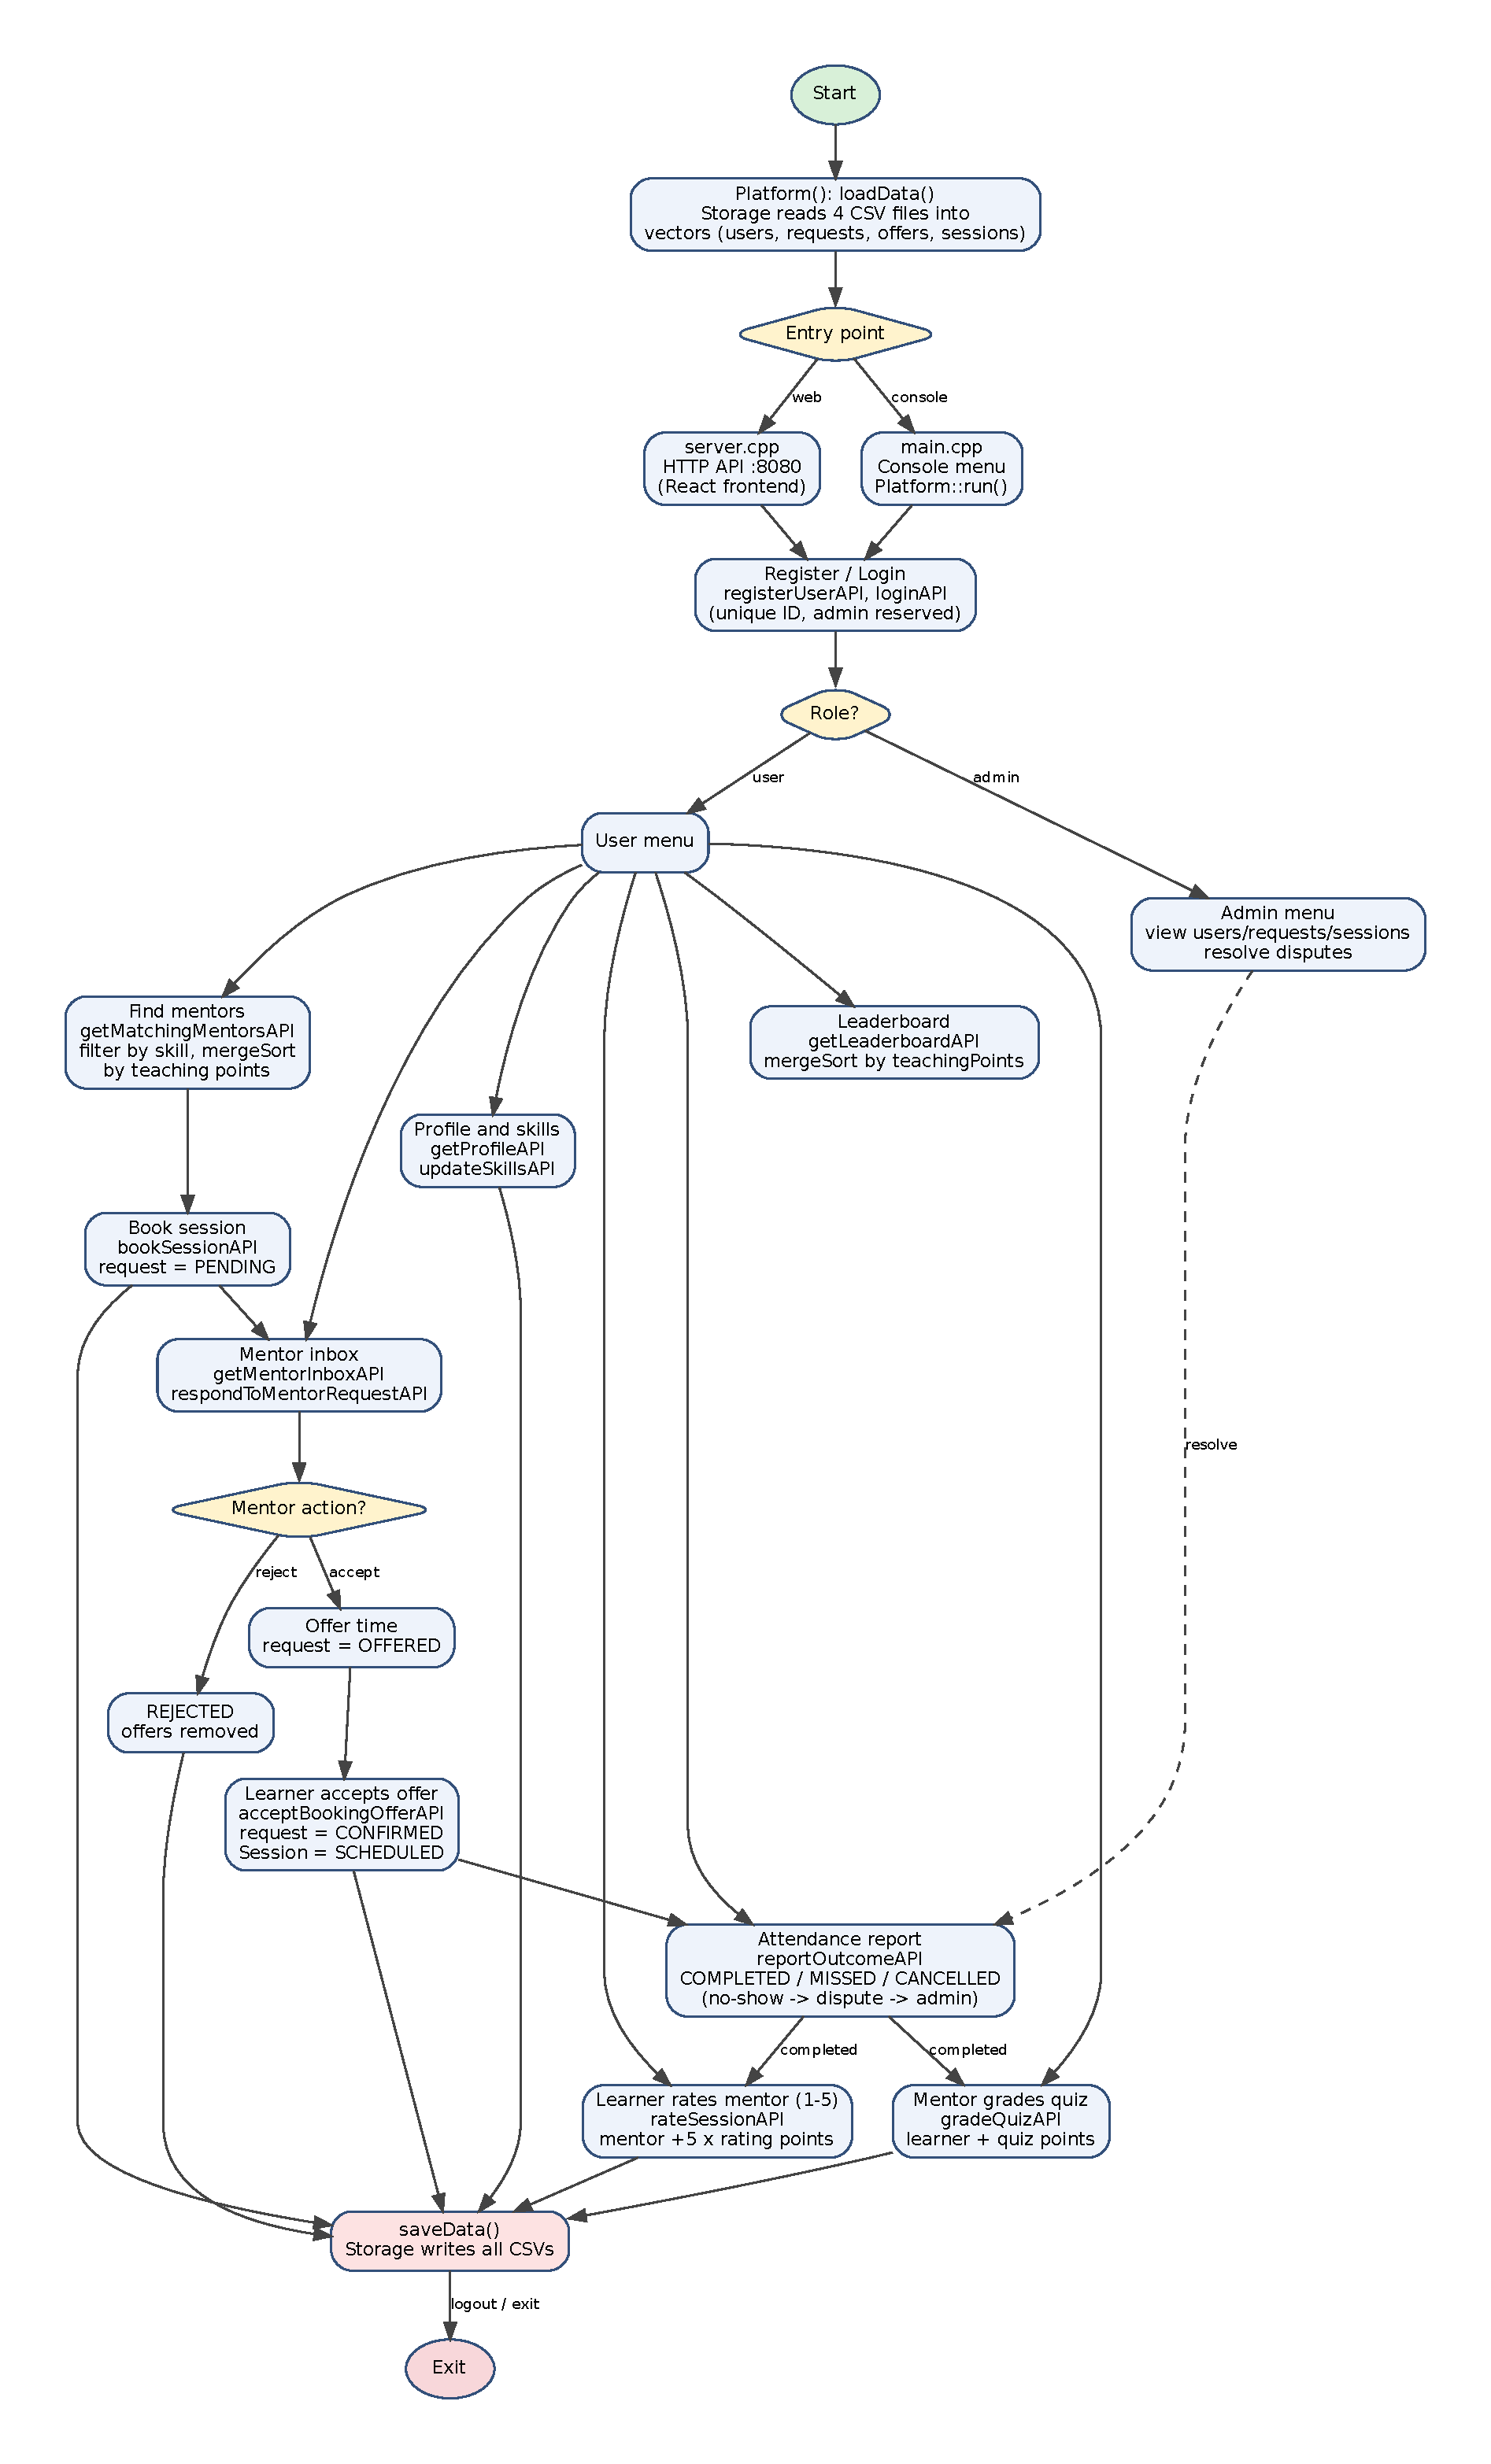
\includegraphics[height=0.88\textheight]{figures/flowchart.pdf}%
}{%
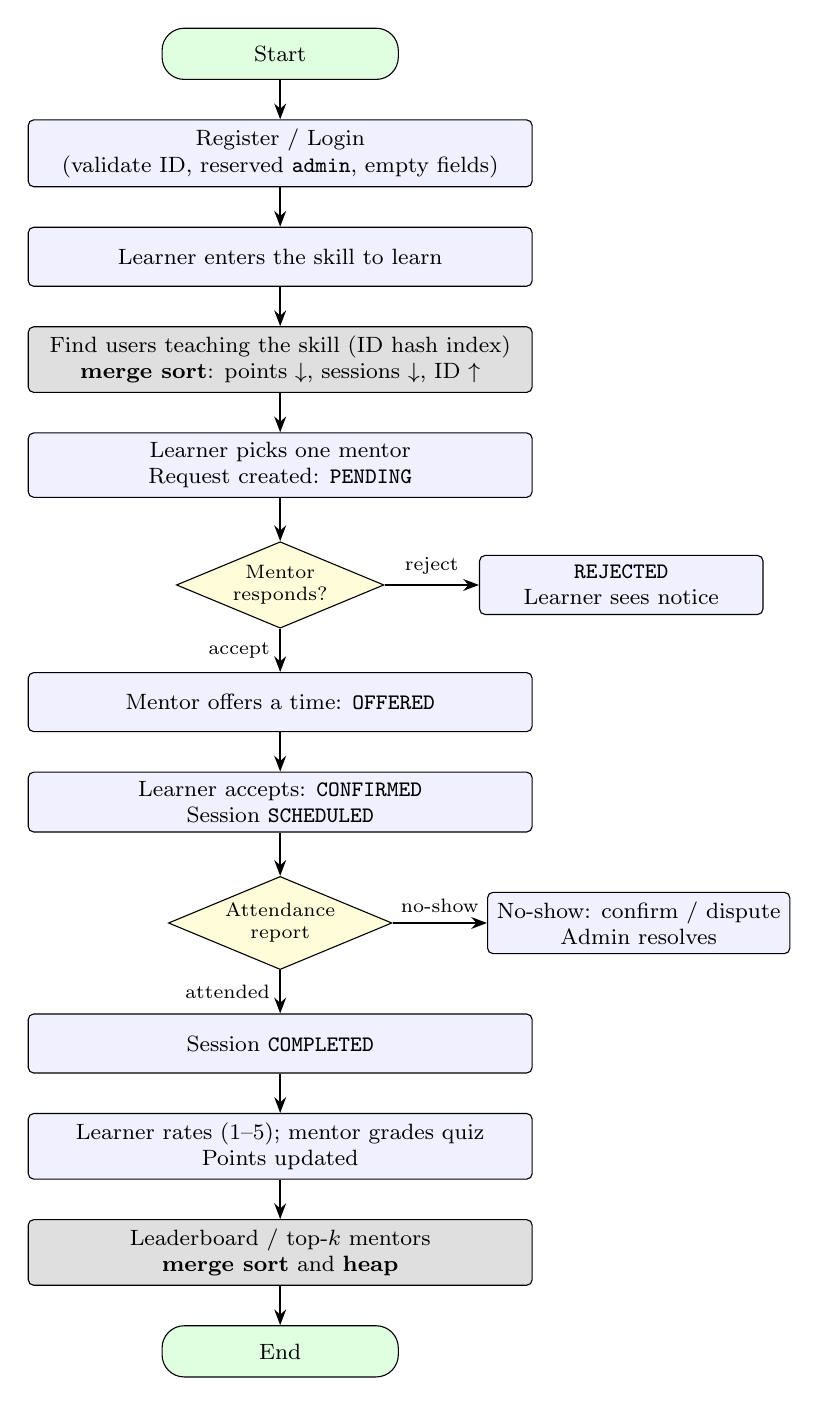
\begin{tikzpicture}[
  node distance=0.5cm,
  proc/.style={draw,rounded corners=2pt,minimum width=6.4cm,minimum height=0.75cm,align=center,font=\footnotesize,fill=blue!6},
  ds/.style={draw,rounded corners=2pt,minimum width=6.4cm,minimum height=0.75cm,align=center,font=\footnotesize,fill=gray!25},
  term/.style={draw,rounded corners=8pt,minimum width=3cm,minimum height=0.65cm,align=center,font=\footnotesize,fill=green!12},
  dec/.style={draw,diamond,aspect=2.4,inner sep=1pt,align=center,font=\scriptsize,fill=yellow!15},
  arr/.style={-{Stealth[length=2mm]},thick},
  lab/.style={font=\scriptsize,midway}]
  \node[term] (start) {Start};
  \node[proc,below=of start] (login) {Register / Login\\(validate ID, reserved \texttt{admin}, empty fields)};
  \node[proc,below=of login] (book) {Learner enters the skill to learn};
  \node[ds,below=of book] (match) {Find users teaching the skill (ID hash index)\\\textbf{merge sort}: points $\downarrow$, sessions $\downarrow$, ID $\uparrow$};
  \node[proc,below=of match] (req) {Learner picks one mentor\\Request created: \texttt{PENDING}};
  \node[dec,below=0.55cm of req] (resp) {Mentor\\responds?};
  \node[proc,right=1.2cm of resp,minimum width=3.6cm] (rej) {\texttt{REJECTED}\\Learner sees notice};
  \node[proc,below=0.55cm of resp] (offer) {Mentor offers a time: \texttt{OFFERED}};
  \node[proc,below=of offer] (acc) {Learner accepts: \texttt{CONFIRMED}\\Session \texttt{SCHEDULED}};
  \node[dec,below=0.55cm of acc] (att) {Attendance\\report};
  \node[proc,right=1.2cm of att,minimum width=3.6cm] (noshow) {No-show: confirm / dispute\\Admin resolves};
  \node[proc,below=0.55cm of att] (done) {Session \texttt{COMPLETED}};
  \node[proc,below=of done] (rate) {Learner rates (1--5); mentor grades quiz\\Points updated};
  \node[ds,below=of rate] (lead) {Leaderboard / top-$k$ mentors\\\textbf{merge sort} and \textbf{heap}};
  \node[term,below=of lead] (end) {End};
  \draw[arr] (start)--(login); \draw[arr] (login)--(book); \draw[arr] (book)--(match);
  \draw[arr] (match)--(req); \draw[arr] (req)--(resp);
  \draw[arr] (resp)--node[lab,above]{reject}(rej);
  \draw[arr] (resp)--node[lab,left]{accept}(offer);
  \draw[arr] (offer)--(acc); \draw[arr] (acc)--(att);
  \draw[arr] (att)--node[lab,above]{no-show}(noshow);
  \draw[arr] (att)--node[lab,left]{attended}(done);
  \draw[arr] (done)--(rate); \draw[arr] (rate)--(lead); \draw[arr] (lead)--(end);
\end{tikzpicture}}
\caption{Flow chart of the Skill Issue platform.}\label{fig:flow}
\end{figure}

\subsection{Idea}
Every user is both a potential \emph{learner} and a potential \emph{mentor}. A learner searches for a skill; the system lists matching mentors ranked by reputation (teaching points). The learner sends a booking request to one mentor, the mentor replies with a time, and the learner confirms. After the session the learner rates the mentor, the mentor grades a short quiz of the learner, and both feed the points that drive the leaderboard.

\subsection{Architecture and modules}
The product is split into seven modules; each has a header (declaration) and a source file (definition).
\begin{description}[leftmargin=1.5cm,style=nextline]
\item[Models (\texttt{models.h})] Plain records \texttt{User}, \texttt{BookingRequest}, \texttt{MentorOffer}, \texttt{BookingDetails} and \texttt{Session}. They carry only data, so every other module can include them without circular dependencies.
\item[Storage (\texttt{storage.h/.cpp})] Class \texttt{Storage} loads and saves the four CSV files (\texttt{users}, \texttt{booking\_requests}, \texttt{mentor\_offers}, \texttt{sessions}). Fields are quoted and escaped, and stray carriage returns (Windows line endings) are ignored when reading; malformed rows are skipped; a missing file is treated as empty data.
\item[Sorting (\texttt{sorting.h})] A templated, stable merge sort taking a comparator. It is used for the leaderboard and mentor ranking.
\item[Hash map (\texttt{hashmap.h})] A self-written hash map (separate chaining, djb2 string hash, doubling when the load factor exceeds 0.75). \texttt{Platform} uses it as an index from user ID and request ID to the position in the corresponding vector, giving $O(1)$ average look-ups.
\item[Priority queue (\texttt{priority\_queue.h})] A self-written binary heap stored in a \texttt{std::vector}, using the same comparator convention as the merge sort. It powers the top-$k$ mentors feature.
\item[Platform (\texttt{platform.h/.cpp})] The core logic. On construction it loads all CSVs into four \texttt{std::vector}s. It also owns the hash indexes \texttt{userIndex\_} and \texttt{requestIndex\_}, which are rebuilt after loading and updated on every registration and booking. Public \texttt{*API} functions (register, login, book, respond, accept, report outcome, rate, grade quiz, leaderboard\ldots) return a success flag and a message and are shared by both interfaces. Every state change calls \texttt{saveData()}.
\item[Interfaces] \texttt{main.cpp} gives a text menu (\texttt{Platform::run}); \texttt{server.cpp} wraps the same \texttt{Platform} in REST endpoints on port 8080 using the third-party header \texttt{cpp-httplib}; the React app in \texttt{frontend/} calls these endpoints.
\end{description}

\subsection{Working of the product}
\paragraph{1. Start-up and authentication.} \texttt{Platform()} reads the CSV files and computes the next free request and session IDs. \texttt{registerUserAPI} rejects empty IDs, the reserved ID \texttt{admin}, and duplicate IDs; \texttt{loginAPI} compares the ID and password.

\paragraph{2. Mentor discovery.} \texttt{getMatchingMentorsAPI(skill, learner)} scans all users, keeps those whose semicolon-separated skill list contains the skill (case-insensitive) and who are not the learner, and sorts them with \texttt{mergeSort}: higher teaching points first, then more teaching sessions, then smaller ID.

\paragraph{3. Booking life-cycle.} A request moves through a small state machine:
\begin{center}\small
\texttt{PENDING} $\xrightarrow{\text{mentor offers a time}}$ \texttt{OFFERED} $\xrightarrow{\text{learner accepts}}$ \texttt{CONFIRMED}\\[3pt]
\texttt{PENDING} or \texttt{OFFERED} $\xrightarrow{\text{mentor rejects}}$ \texttt{REJECTED}
\end{center}
\texttt{book\-Session\-API} validates mentor, learner and skill and creates the request. \texttt{respondToMentor\-Request\-API} lets \emph{only the targeted mentor} reject (which also deletes its offers) or offer a time. \texttt{accept\-Booking\-Offer\-API} turns the offer into a confirmed time, creates a \texttt{SCHEDULED} \texttt{Session} and increments the teaching/learning counters.

\paragraph{4. Attendance and disputes.} After the scheduled time the participants report the outcome. In the console flow, a no-show report puts the session in \texttt{AWAITING\_CONFIRMATION}; the other side can agree (5 points are deducted from the absentee) or disagree, which sets \texttt{DISPUTED} for the admin to resolve (completed, learner absent, mentor absent, or reschedule).

\paragraph{Top mentors (heap).} \texttt{getTopMentorsAPI(k)} keeps a heap of at most $k$ users whose top element is the \emph{worst} user kept so far. Each user is pushed and, if the heap exceeds $k$, the worst is popped, so the cost is $O(n\log k)$ instead of sorting all $n$ users. The result is reversed to give best-first order and is exposed as \texttt{GET /api/top-mentors?k=3}.

\paragraph{5. Points and leaderboard.} A learner rating $r\in[1,5]$ gives the mentor $5r$ teaching points (console flow); the mentor's quiz mark adds to the learner's total points. \texttt{getLeaderboardAPI} sorts all users by teaching points (ties by ID) and strips passwords before returning them.

\subsection{Data structures and complexity}
\begin{center}\begin{tabular}{p{3.8cm}p{5.2cm}p{4.2cm}}\toprule
Structure / algorithm & Used for & Cost\\\midrule
\texttt{std::vector} of records & In-memory tables for users, requests, offers, sessions & append $O(1)$ amortised\\
Hash map (own implementation) & \texttt{findUser}, \texttt{findRequest} through ID indexes & $O(1)$ average, $O(n)$ rebuild on load\\
Binary heap / priority queue (own) & Top-$k$ mentors & push/pop $O(\log k)$, top-$k$ in $O(n\log k)$\\
Merge sort (own implementation) & Leaderboard, mentor ranking & $O(n\log n)$, $O(n)$ extra space, stable\\
Erase--remove idiom & Deleting offers of a rejected request & $O(n)$\\
String tokenising (\texttt{;}) & Skill matching & $O(L)$ per user\\
State machine on strings & Request and session status & $O(1)$ per transition\\
CSV (flat file) & Persistence & $O(n)$ per save\\\bottomrule
\end{tabular}\end{center}
Users and requests are only ever appended, never deleted, so the hash indexes only need insertions and a rebuild after loading; positions never shift. Linear scans remain for offers and sessions, which are filtered by several fields rather than looked up by one key.

%=====================================================================
\section{Step 3 -- Coding}
\subsection{Directory structure}
\begin{lstlisting}[language={},numbers=none]
All_Hs_106125037_106125039_106125041_CSLR31_Project/
|-- Makefile          a.out (console)  server (HTTP API)
|-- include/          models.h storage.h platform.h sorting.h hashmap.h
|                     priority_queue.h httplib.h
|-- Source/           main.cpp platform.cpp storage.cpp server.cpp
|-- object/           *.o files
|-- data/             users.csv booking_requests.csv mentor_offers.csv sessions.csv
|-- Test/             test_skill_issue.cpp testdata/
|-- frontend/         React + Vite web UI
|-- Document/         report.tex, user_manual.md, figures/
`-- Video/            project experience video
\end{lstlisting}
Build with \texttt{make}; run \texttt{./a.out} (console) or \texttt{./server} then \texttt{npm run dev} in \texttt{frontend/}. Declarations live in the \texttt{.h} files and definitions in the \texttt{.cpp} files, as required.

\subsection{Sample code}
Generic stable merge sort (\texttt{include/sorting.h}):
\begin{lstlisting}
template <typename T, typename Compare>
void mergeSortHelper(std::vector<T>& arr, int left, int right, Compare comp) {
    if (left >= right) return;
    int mid = left + (right - left) / 2;
    mergeSortHelper(arr, left, mid, comp);
    mergeSortHelper(arr, mid + 1, right, comp);
    std::vector<T> temp;
    int i = left, j = mid + 1;
    while (i <= mid && j <= right) {
        if (!comp(arr[j], arr[i])) temp.push_back(arr[i++]);  // keeps ties stable
        else                       temp.push_back(arr[j++]);
    }
    while (i <= mid)   temp.push_back(arr[i++]);
    while (j <= right) temp.push_back(arr[j++]);
    for (int k = 0; k < (int)temp.size(); k++) arr[left + k] = temp[k];
}
\end{lstlisting}
Use in \texttt{getMatchingMentorsAPI} (\texttt{Source/platform.cpp}):
\begin{lstlisting}
mergeSort(mentors, [](const User& a, const User& b) {
    if (a.teachingPoints != b.teachingPoints) return a.teachingPoints > b.teachingPoints;
    if (a.teachingSessions != b.teachingSessions) return a.teachingSessions > b.teachingSessions;
    return a.id < b.id;
});
\end{lstlisting}
Core of the self-written hash map (\texttt{include/hashmap.h}):
\begin{lstlisting}
void put(const K& key, const V& value) {
    Node* node = findNode(key);
    if (node) { node->value = value; return; }            // overwrite existing key
    if (size_ + 1 > bucketCount_ * 3 / 4) resize(bucketCount_ * 2);  // keep chains short
    std::size_t b = hashKey(key) % bucketCount_;
    buckets_[b] = new Node{key, value, buckets_[b]};      // insert at chain head
    ++size_;
}
\end{lstlisting}
Core of the self-written priority queue (\texttt{include/priority\_queue.h}):
\begin{lstlisting}
void push(const T& value) { data_.push_back(value); siftUp(data_.size() - 1); }
void pop() {
    data_.front() = data_.back();      // move last leaf to the root
    data_.pop_back();
    if (!data_.empty()) siftDown(0);
}
\end{lstlisting}
The project compiles with \texttt{-std=c++17 -Wall -Wextra -pedantic} without warnings.

\subsection{Known limitations}
\begin{itemize}[nosep]
\item The API versions \texttt{rateSessionAPI} and \texttt{gradeQuizAPI} (used by the web app) store the rating/score but do not add the points that the console versions add; the quiz range is 0--100 in the API but 0--5 in the console.
\item The API reports only the mentor's outcome; the dispute flow exists only in the console.
\item Passwords are stored in plain text; the server trusts the user ID sent by the client (no session tokens).
\end{itemize}

%=====================================================================
\section{Step 4 -- Testing}
Tests are in \texttt{Test/test\_skill\_issue.cpp}; run \texttt{make test}. They use their own data (\texttt{Test/testdata}) copied to a temporary directory, so real data is never modified. \textbf{Result: 73 passed, 0 failed}.

\paragraph{Test data.} Five users: u1 (C++, Python; 40 pts, 3 sessions), u2 (Python, Web; 40 pts, 5 sessions), u3 (Python; 10 pts), u4 (Dance; 0 pts), u5 (Java; 25 pts).
\begin{center}\small\begin{tabular}{p{2cm}p{6.4cm}p{5cm}}\toprule
IDs & Scenario & Expected\\\midrule
TC01--05 & Register valid / duplicate / reserved \texttt{admin} / empty ID / empty password & Only the valid one succeeds\\
TC06--12 & Login right/wrong/unknown; profile; update skills & Correct accept/reject; password hidden\\
TC13--16 & Mentor search for ``python'' by u5, by u1, unknown learner, untaught skill & Order u2,u1,u3 (tie on points broken by sessions); self excluded; empty lists\\
TC17--18 & Leaderboard & u1,u2,u5\ldots; passwords blank\\
TC19--22 & Booking: unknown mentor, self, skill not taught, valid & First three fail, last succeeds\\
TC23--30 & Inbox and mentor response: target vs other mentor, bad action, no time, duplicate offer & Only target mentor can offer once\\
TC31--36 & Learner accepts offer: wrong learner, wrong mentor, twice, counters & Session created once; counters $+1$\\
TC37--46 & Outcome and rating: rating too early, bad outcome, wrong user, 0/6, double rating & Rejected except valid actions\\
TC47--50 & Quiz grading: 101, non-mentor, valid, unknown session & Only valid succeeds\\
TC51--53 & Reject flow & Request leaves inbox, cannot be accepted\\
TC54--55 & Restart persistence & New user and sessions reloaded from CSV\\
TC56--59 & Merge sort: empty, single, ascending, stable, 2000 random vs \texttt{std::stable\_sort} & Identical results\\
TC60--64 & Hash map: 1000 inserts with repeated resizing, overwrite, missing key, remove, integer keys & All keys found; size correct\\
TC65--67 & Priority queue: empty queue, \texttt{top()} on empty (exception), push 7 values & Popped in priority order 9,9,7,5,3,2,1\\
TC68--71 & Top-$k$ mentors: $k=2$, $k$ larger than users, $k\le0$, agreement with leaderboard & Correct best-first order; empty for $k\le0$\\
TC72--73 & CSV files with Windows (CRLF) line endings and a stray carriage return inside quoted values & Loaded cleanly; no hidden CR in IDs or times\\\bottomrule
\end{tabular}\end{center}
\paragraph{Manual testing.} The HTTP endpoints were additionally checked by hand with \texttt{curl} against the running server: registration (valid, duplicate, reserved, empty password), login, mentor search with a points tie, the full booking path (request, offer, acceptance, repeated acceptance), rating before and after completion, out-of-range ratings, quiz grading by a non-mentor, profile of an unknown user, and persistence of the rating and quiz values in \texttt{sessions.csv}. All 31 checks behaved as specified; the one finding was that a non-numeric numeric parameter (for example \texttt{requestId=abc}) raises an uncaught \texttt{std::stoi} exception and returns HTTP~500 instead of 400.
\paragraph{Not automatically tested.} The interactive console menus, dispute resolution and the React UI.

%=====================================================================
\section{Step 5 -- Contributions, Key Takeaways, Future Scope, Acknowledgements and References}
\subsection{Individual contributions}
The work was divided by area at the start of the project. The table states what each member's area produced in the delivered code; ideas planned for an area but not completed are listed under Future Scope and are not claimed here.
% VERIFY BEFORE SUBMITTING: make each row match what that person really wrote and can explain in the viva.
\begin{center}\small\begin{tabular}{p{3.3cm}p{3.6cm}p{7.6cm}}\toprule
Member & Assigned area & Contribution in the delivered code\\\midrule
\textbf{Himani}\newline 106125041 & Skill discovery and matching &
  Skill-list handling and case-insensitive skill matching; matching-mentor search and its three-level ranking; update-teaching-skills feature; mentor-selection step of the booking flow; \emph{Book a Session} and \emph{Update Skills} pages of the web UI.\\[4pt]
\textbf{Harsh}\newline 106125039 & Points, ranking and priority structures &
  Generic merge sort (\texttt{sorting.h}) and comparators; teaching leaderboard; own hash map (\texttt{hashmap.h}) and binary-heap priority queue (\texttt{priority\_queue.h}); top-$k$ mentors; teaching points from ratings, learner points from quiz marks, no-show penalties.\\[4pt]
\textbf{Harini}\newline 106125037 & Booking life-cycle, sessions and persistence &
  Booking request, offer and confirmation flow; session records and states; attendance reporting, no-show confirmation, dispute and admin resolution; CSV storage layer (\texttt{storage.cpp}); REST server (\texttt{server.cpp}); project integration, Makefile and testing.\\\bottomrule
\end{tabular}\end{center}
All three members took part in design discussions, testing and final integration of the console application, REST API and web UI.

\subsection{Key takeaways}
\begin{itemize}
\item Separating declarations (\texttt{.h}) from definitions (\texttt{.cpp}) let three people work on modules in parallel and kept the build incremental through a Makefile.
\item A templated merge sort with a comparator gave one reusable, stable $O(n\log n)$ ranking routine for three different orderings.
\item Modelling booking and session status as an explicit state machine made invalid actions (double accept, double rating) easy to detect and test.
\item Implementing our own hash map and binary heap showed how chaining, load-factor resizing and sift-up/sift-down give $O(1)$ look-ups and $O(\log n)$ priority operations.
\item Keeping one \texttt{Platform} class behind both a console UI and a REST API avoids duplicated rules, but it also showed what happens when the two paths drift apart (the point-awarding mismatch); automated tests exposed edge cases (ties, empty inputs, persistence) that manual clicking missed.
\end{itemize}

\subsection{Future scope}\label{sec:future}
\begin{itemize}[nosep]
\item \textbf{Planned but not implemented:} a skill graph (user$\leftrightarrow$skill and skill$\leftrightarrow$skill adjacency lists) with BFS/DFS for ``who can teach X'' and compatibility scoring; a trie for skill-name autocomplete; interval scheduling for slot-conflict detection and timetable overlap; a queue that serves booking requests in priority order using the heap.
\item Index offers and sessions by key as well (currently only users and requests use the hash map), and let a heap order the mentor inbox by urgency.
\item Hash passwords and add token-based sessions.
\item Detect overlapping appointments; add notifications; use a real database; port the dispute flow to the API; mobile app.
\end{itemize}

\subsection{Acknowledgements}
We thank our course instructor for the project framework and guidance, the Department of Computer Science and Engineering, NIT Tiruchirappalli, for the laboratory facilities, and the authors of the open-source tools we used: cpp-httplib, React, Vite, Graphviz and \LaTeX{} (Overleaf).

\subsection{References}
\begin{enumerate}[nosep]
\item T.~H.~Cormen et al., \emph{Introduction to Algorithms}, 4th ed., MIT Press, 2022 (merge sort).
\item cpp-httplib, a C++ single-header HTTP library, \url{https://github.com/yhirose/cpp-httplib} (third-party code in \texttt{include/httplib.h}, not written by the team).
\item cppreference.com, C++17 standard library documentation, \url{https://en.cppreference.com}.
\item UNESCO/UN Sustainable Development Goals, \url{https://www.unesco.org/en/sdgs}.
\item React and Vite documentation, \url{https://react.dev}, \url{https://vite.dev}.
\item Graphviz, \url{https://graphviz.org} (flow chart generation).
\end{enumerate}
\end{document}
